\chapter{Arquitectura i Disseny}
\label{ch:arquitectura}

L'arquitectura de \textit{Web Core View} s'ha dissenyat sota els principis de modularitat, escalabilitat i eficiència en el consum de recursos. Atès que el software s'executa en un entorn \textit{embedded} (el videogravador), s'ha optat per una arquitectura desacoblada on el \textit{frontend} assumeix la major part de la lògica de presentació per alliberar la CPU del maquinari per a les tasques crítiques de seguretat.

\section{Arquitectura Global del Sistema}

L'ecosistema del videogravador (NVR) de Lanaccess es basa en un model de microserveis interns coordinats dins del sistema operatiu del gravador. La plataforma interactua amb els següents serveis crítics executant-se en l'entorn \textit{embedded}:

\begin{itemize}
    \item \textbf{la-core-legacy:} El nucli central del sistema. Gestiona la configuració del gravador (API REST), l'autenticació i autorització d'usuaris, els bloquejos de recursos (\textit{locks}) i la coordinació del cicle de vida de la resta de serveis.
    \item \textbf{la-video-engine:} El motor de vídeo. Processa els fluxos de les càmeres IP, els grava als discos i els redistribueix cap a \textbf{MediaMTX} per a la seva servei en temps real. És l'únic servei del sistema amb privilegis d'escriptura a disc, centralitzant i controlant totes les operacions d'E/S.
    \item \textbf{la-db-engine:} Passarel·la de persistència lògica. Implementa un \textit{Virtual File System} (VFS) personalitzat de SQLite que, en lloc d'operar sobre fitxers físics, redirigeix totes les lectures i escriptures a través de \textit{sockets} Unix cap a \textbf{la-video-engine}. Exposa una interfície \textbf{gRPC} als seus clients i no té permisos directes sobre el disc.
    \item \textbf{la-core-notifier:} Passarel·la de WebSockets per a notificacions generals del sistema. Es subscriu al bus \textbf{D-Bus} per detectar esdeveniments de maquinari —com pèrdues de senyal de vídeo o canvis d'estat de càmera— i els retransmet immediatament al \textit{frontend} via WSS.
    \item \textbf{la-core-alarm:} Passarel·la de WebSockets especialitzada en alarmes. Es comunica amb \textbf{la-db-engine} via \textbf{gRPC} per persistir els registres d'events, i escolta el \textbf{D-Bus} per detectar activacions de sensors i relés, transmetent-les en temps real al client.
    \item \textbf{MediaMTX:} Servidor de mitjana de codi obert que actua com a motor de \textit{streaming} de vídeo en temps real. Rep els fluxos de les càmeres des de \textbf{la-video-engine} i els redistribueix als clients via dos protocols diferenciats: \textbf{WebRTC} (transport SRTP/UDP negociat per ICE), i \textbf{HLS} (\textit{HTTP Live Streaming}).
\end{itemize}

Aquests serveis es relacionen entre ells mitjançant diferents protocols i busos de comunicació per garantir un rendiment òptim. Tal com s'il·lustra en el diagrama de la Figura \ref{fig:arquitectura_serveis}, el \textit{frontend} (\textit{web core view}) interactua amb el backend principalment per dues vies: peticions HTTPS cap a \textbf{la-core-legacy}, i connexions de WebSockets segurs (\textit{wss}) cap a \textbf{la-core-notifier} i \textbf{la-core-alarm} per rebre notificacions en temps real.

Internament, els microserveis intercanvien informació majoritàriament a través del \textbf{D-Bus} de Linux. Per exemple, quan hi ha un canvi d'estat a nivell de maquinari (com una alarma), es publica al \textit{D-Bus}. Els serveis \textbf{la-core-notifier} i \textbf{la-core-alarm} estan subscrits a aquest bus i, en rebre el senyal, transmeten l'esdeveniment via WebSockets al \textit{frontend}. D'altra banda, \textbf{la-core-alarm} utilitza crides \textbf{gRPC} per comunicar-se de manera ràpida i eficient amb \textbf{la-db-engine}.

\textbf{la-db-engine} intercepta la lectura i escriptura d'alarmes a disc implementant un \textit{Virtual File System} (VFS) personalitzat de SQLite: en lloc de realitzar les operacions d'E/S sobre fitxers físics, redirigeix totes les escriptures i lectures de SQLite a través de \textit{sockets} Unix cap a \textbf{la-video-engine}. D'aquesta manera, \textbf{la-db-engine} presenta una base de dades lògica als seus clients (via gRPC), però no té permisos ni responsabilitat sobre el disc. \textbf{la-video-engine} és l'únic servei amb privilegis per escriure a disc, cosa que centralitza i controla totes les operacions d'E/S del sistema.

Cal destacar que tots aquests microserveis —\textbf{la-core-legacy}, \textbf{la-video-engine}, \textbf{la-db-engine}, \textbf{la-core-notifier} i \textbf{la-core-alarm}— estan definits i gestionats com a \textbf{unitats de \textit{systemd}} al sistema operatiu del gravador. Cadascun d'ells disposa del seu propi fitxer \texttt{.service}, que defineix les dependències d'arrencada, les polítiques de reinici automàtic i els límits de recursos. Això significa que l'operador pot gestionar el cicle de vida de qualsevol servei de forma independent amb \texttt{systemctl} (per exemple, \texttt{systemctl restart la-db-engine}), i que \textit{systemd} s'encarrega de garantir que els serveis s'arrenquen en l'ordre correcte i es recuperen automàticament en cas de fallada.

\begin{figure}[htbp]
  \centering
  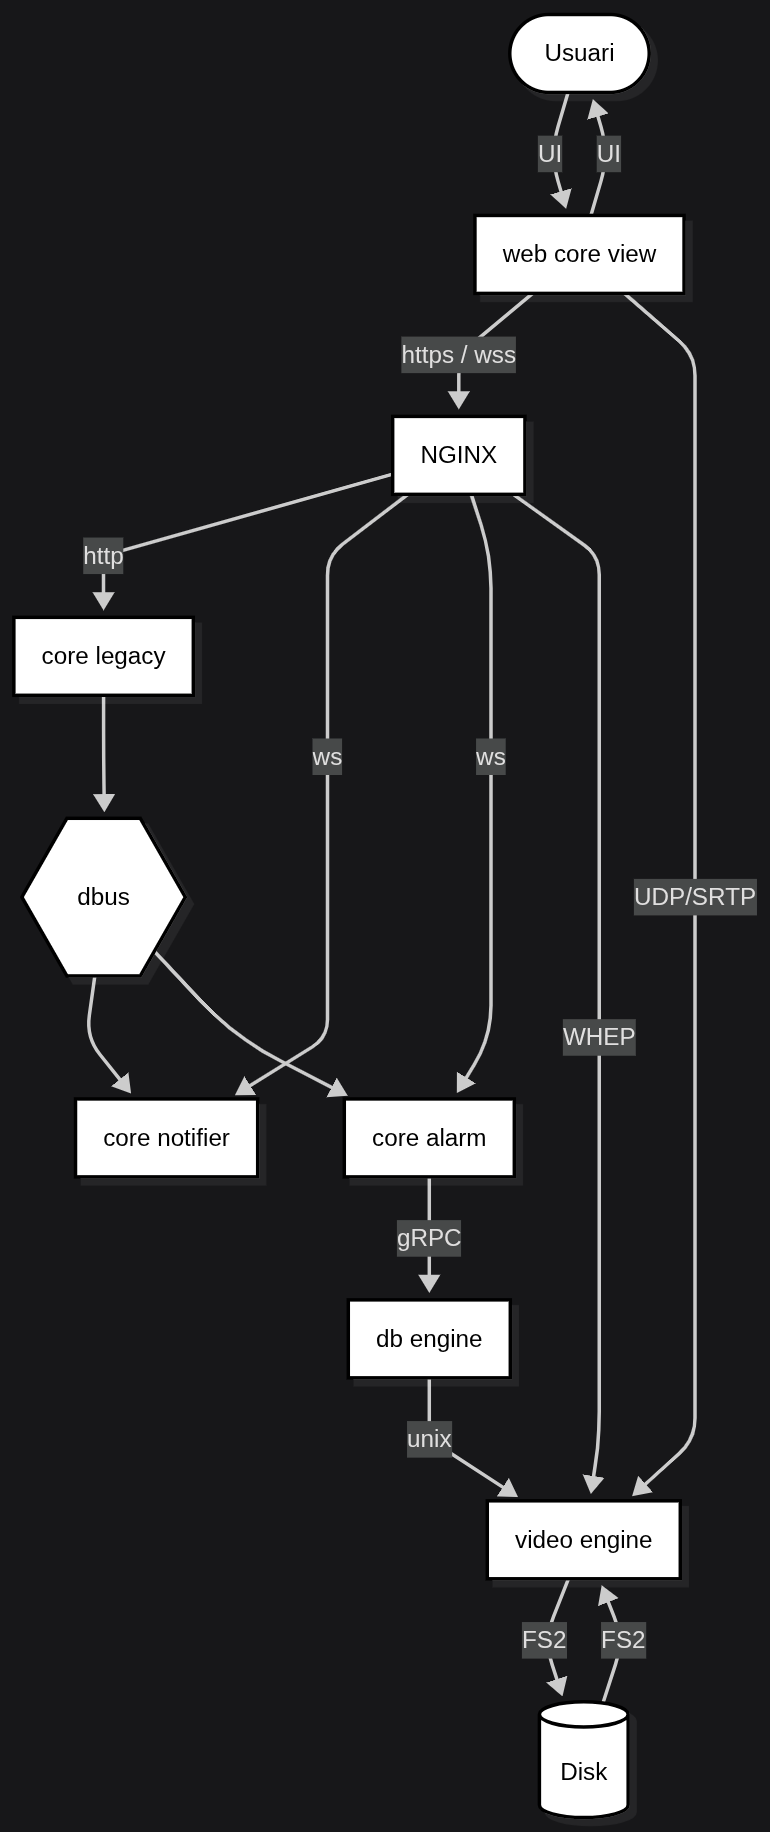
\includegraphics[width=0.9\textwidth, height=0.85\textheight, keepaspectratio]{figures/diagrames/arquitectura_serveis.png}
  \caption{Relació i comunicació entre els serveis de l'NVR.}
  \label{fig:arquitectura_serveis}
  \small Font: Elaboració pròpia.
\end{figure}

\clearpage
\subsection{Capa de comunicació i Proxy}

Per comunicar la web amb els serveis de manera segura, s'interposa \textbf{NGINX} com a \textit{proxy} invers i porta d'entrada única (\textit{gateway}) al sistema. NGINX escolta als ports \texttt{60080} (HTTP) i \texttt{60443} (HTTPS/SSL), i assumeix quatre responsabilitats principals: gestiona el xifratge TLS (protocols TLSv1.2 i TLSv1.3, xifrat \texttt{EECDH+AESGCM}), aplica capçaleres de seguretat HTTP (\texttt{Strict-Transport-Security}, \texttt{X-Frame-Options: SAMEORIGIN}, \texttt{X-Content-Type-Options: nosniff}), controla l'autenticació de les rutes protegides mitjançant el mecanisme intern \texttt{auth\_request}, i enruta cada petició cap al microservei intern corresponent en funció de la ruta URL. Des del punt de vista del navegador, tots els serveis queden amagats darrere una única adreça.

La configuració NGINX agrupa les rutes en quatre blocs funcionals:

\begin{itemize}
    \item \textbf{Configuració i control (HTTPS):} La gran majoria de les rutes —\texttt{/api.rest/}, \texttt{/webprotocol/}, \texttt{/onvif/}, \texttt{/device-service/} i els nombrosos \textit{endpoints} \texttt{.cgi}— es deriven cap a \textbf{la-core-legacy} (port intern \texttt{60088}). Aquest servei centralitza la gestió de la configuració, l'autenticació i el control del sistema.

    \item \textbf{Canals de temps real (WSS):} Les connexions WebSocket persistents segueixen dues rutes diferenciades: \texttt{/ws/la-core-notifier/} es deriven cap al port \texttt{60070} (\textbf{la-core-notifier}), i \texttt{/ws/la-core-alarm/} cap al port \texttt{60071} (\textbf{la-core-alarm}). Ambdós serveis envien esdeveniments en temps real al \textit{frontend} —pèrdues de vídeo, activació de relés, alarmes de sensor— sense que el client hagi de fer \textit{polling}.

    \item \textbf{Vídeo en temps real:} S'ofereixen dos mecanismes de \textit{streaming} gestionats per \textbf{MediaMTX}: el camí \texttt{/stream/} (port \texttt{60889}) serveix vídeo via WebRTC, amb senyalització sobre WebSocket i transport de mitjana SRTP/UDP negociat per ICE; el camí \texttt{/hls/} (port \texttt{60888}) serveix el mateix vídeo en format HLS per a clients que no suporten o tenen dificultats amb WebRTC. 

    \item \textbf{Serveis auxiliars:} El camí \texttt{/video-engine/} enruta directament cap a \textbf{la-video-engine} (port \texttt{60890}) per a operacions de control i consulta del motor de vídeo. El camí \texttt{/db-engine/} connecta amb \textbf{la-db-engine} (port \texttt{60891}) per a consultes de dades històriques. El camí \texttt{/terminal/} connecta amb el servei \textbf{ttyd} (port \texttt{7681}), que ofereix una terminal interactiva accessible directament des del navegador.
\end{itemize}

Per tal de sintetitzar la interacció entre els components, a la Taula \ref{tab:matriu_comunicacio} es detallen els protocols i la naturalesa del trànsit entre el navegador i el gravador:

\begin{table}[htbp]
  \centering
  \caption{Matriu de comunicació de la plataforma.}
  \label{tab:matriu_comunicacio}
  \resizebox{\textwidth}{!}{
  \begin{tabular}{@{}lllll@{}}
    \toprule
    \textbf{Origen} & \textbf{Destinació (Servei)} & \textbf{Ruta NGINX} & \textbf{Protocol} & \textbf{Finalitat} \\ \midrule
    Navegador & NGINX $\rightarrow$ \textbf{la-core-legacy} & \texttt{/login/}, \texttt{/(en|es|fr)/} & HTTPS & Descàrrega de l'aplicació Angular (SPA) \\
    Navegador & NGINX $\rightarrow$ \textbf{la-core-legacy} & \texttt{/api.rest/}, \texttt{/webprotocol/}, \texttt{*.cgi} & HTTPS & Configuració, autenticació i control del sistema \\
    Navegador & NGINX $\rightarrow$ \textbf{la-core-notifier} & \texttt{/ws/la-core-notifier/} & WSS & Notificacions de sistema en temps real \\
    Navegador & NGINX $\rightarrow$ \textbf{la-core-alarm} & \texttt{/ws/la-core-alarm/} & WSS & Notificacions d'alarmes en temps real \\
    Navegador & NGINX $\rightarrow$ \textbf{MediaMTX} & \texttt{/stream/} & WSS + SRTP/UDP & Vídeo en directe via WebRTC \\
    Navegador & NGINX $\rightarrow$ \textbf{MediaMTX} & \texttt{/hls/} & HTTPS & Vídeo en directe via HLS \\
    Navegador & NGINX $\rightarrow$ \textbf{la-video-engine} & \texttt{/video-engine/} & HTTPS & Control i consulta del motor de vídeo \\
    Navegador & NGINX $\rightarrow$ \textbf{la-db-engine} & \texttt{/db-engine/} & HTTPS & Consultes de dades històriques \\
    Navegador & NGINX $\rightarrow$ \textbf{ttyd} & \texttt{/terminal/} & WSS & Terminal interactiva via navegador \\
    % \textbf{la-core-notifier} / \textbf{la-core-alarm} & \textbf{la-db-engine} & — & gRPC / D-Bus & Comunicació interna del backend \\
    % \textbf{la-video-engine} & \textbf{la-db-engine} & — & Unix Sockets & Persistència al disc (VFS SQLite) \\ \bottomrule
  \end{tabular}
  }
\end{table}

\clearpage
El Llistat \ref{lst:nginx_routing} mostra els blocs de configuració NGINX que implementen les rutes principals de la plataforma, extrets directament del fitxer \texttt{la-core.conf} del repositori de build \textbf{mantos-rec} (\texttt{sources/meta-mantos/recipes-httpd/nginx/nginx/la-core.conf}):

\begin{lstlisting}[language=bash, label={lst:nginx_routing}, caption={Fragment de la configuració NGINX (la-core.conf, repositori mantos-rec): rutes principals de la plataforma.}]
# Aplicacio Angular (SPA) - requereix autenticacio
location ~ ^/(en|es|fr)/ {
    auth_request /auth.cgi;
    error_page 401 = @error401;
    alias /data/web-core-view/var/www/browser/;
    try_files $uri $uri/ /login/index.html;
}

# WebSocket - Notificacions generals del sistema
location /ws/la-core-notifier/ {
    proxy_pass http://localhost:60070/;
    proxy_http_version 1.1;
    proxy_set_header Upgrade $http_upgrade;
    proxy_set_header Connection "upgrade";
    proxy_send_timeout 600s;
    proxy_read_timeout 600s;
}

# WebSocket - Canal d'alarmes
location /ws/la-core-alarm/ {
    proxy_pass http://localhost:60071/;
    proxy_http_version 1.1;
    proxy_set_header Upgrade $http_upgrade;
    proxy_set_header Connection "upgrade";
    proxy_send_timeout 600s;
    proxy_read_timeout 600s;
}

# Motor de video - control i consulta (protegit per auth)
location /video-engine/ {
    auth_request /auth.cgi;
    error_page 401 = @error401;
    proxy_http_version 1.1;
    proxy_pass http://localhost:60890/;
}

# Base de dades - dades historiques (protegit per auth)
location /db-engine/ {
    auth_request /auth.cgi;
    error_page 401 = @error401;
    proxy_http_version 1.1;
    proxy_pass http://localhost:60891/;
}

# Streaming WebRTC via MediaMTX (protegit per auth)
location /stream/ {
    auth_request /auth.cgi;
    error_page 401 = @error401;
    proxy_pass http://localhost:60889/stream/;
    proxy_http_version 1.1;
    proxy_set_header Upgrade $http_upgrade;
    proxy_set_header Connection "upgrade";
}
\end{lstlisting}

% Per resoldre aquest desacoblament a l'hora d'enviar esdeveniments, s'ha dissenyat un mecanisme de \textbf{bridging de protocols (Protocol Bridging)} centralitzat en el servei de notificacions (\textit{Core Notifier}) del gravador. Aquest servei actua com a intermediari actiu (\textit{gateway}): es subscriu als esdeveniments de sistema (com pèrdues de vídeo o activació de relés) mitjançant el bus D-Bus i canals gRPC, tradueix aquestes estructures de baix nivell en missatges JSON lleugers i, finalment, els transmet en temps real pel canal de \textbf{WebSockets} (WSS) \cite{rfc6455} fins al client Angular. Aquest disseny garanteix que el frontend pugui respondre immediatament a qualsevol esdeveniment de seguretat, sense connexions binàries natives costoses ni sobrecàrrega de la CPU del client.

\clearpage
\subsection{Seguretat Defensiva contra vectors d'atac OWASP}
Com a requisit no funcional de seguretat crítica, el frontend s'ha dissenyat per mitigar de forma activa les principals vulnerabilitats del catàleg OWASP Top 10. La gestió de la sessió s'ha dissenyat per eliminar tots els vectors de robatori de credencials: les \textit{cookies} de sessió es gestionen amb els atributs \texttt{HttpOnly} i \texttt{Secure} configurats exclusivament a la capa de NGINX, de manera que resten completament inaccessibles des de qualsevol codi JavaScript del client i, per tant, immunitzades contra atacs de tipus \textit{Cross-Site Scripting} (XSS). La prevenció de \textit{Cross-Site Request Forgery} (CSRF) s'aconsegueix gràcies a la política \textit{Same-Origin} imposada per NGINX i a la naturalesa \textit{zero-persistence} del Signal privat d'estat en memòria del \textit{frontend}: un recarregament de pàgina invalida la sessió al costat del client sense necessitat de cap \textit{token} CSRF addicional.

Addicionalment, a la capa de NGINX, s'ha unificat l'origen de l'aplicació i l'API REST sota un mateix servidor de recursos, cosa que permet aplicar polítiques de \textit{Same-Origin} estrictes que limiten els vectors d'injeccions \textit{Cross-Site Scripting} (XSS) i els intents de \textit{Clickjacking}.

L'ús de NGINX com a \textit{entry point} és indispensable per a la seguretat del sistema. En centralitzar les peticions, NGINX actua de tallafoc per als serveis \textbf{la-video-engine} i \textbf{la-core-legacy}, impedint l'accés directe als ports interns. A més, permet que el token JWT generat per l'autenticació sigui vàlid per a tots els microserveis sota un mateix domini de seguretat, simplificant la gestió de capçaleres \textit{Authorization} i evitant problemes de CORS (Cross-Origin Resource Sharing) que podrien bloquejar l'streaming de vídeo.

\begin{lstlisting}[language=bash, label={lst:nginx_security}, caption={Fragment de la configuració NGINX (la-core.conf): TLS i capçaleres de seguretat HTTP.}]
server {
    listen 60080;
    listen 60443 ssl;

    # Certificats TLS del dispositiu
    ssl_certificate     /etc/ssl/certs/la-certificate.crt;
    ssl_certificate_key /etc/ssl/private/la-certificate.key;

    # Protocols i xifrats forts (OWASP TLS Cheat Sheet)
    ssl_protocols             TLSv1.2 TLSv1.3;
    ssl_prefer_server_ciphers on;
    ssl_dhparam               /etc/nginx/la-dhparam.pem;
    ssl_ciphers               EECDH+AESGCM:EDH+AESGCM;
    ssl_ecdh_curve            secp384r1;
    ssl_session_timeout       10m;
    ssl_session_cache         shared:SSL:10m;
    ssl_session_tickets       off;
    ssl_stapling              on;
    ssl_stapling_verify       on;

    # Capçaleres de seguretat HTTP
    add_header Strict-Transport-Security
               "max-age=31536000; includeSubDomains" always;
    add_header X-Frame-Options        "SAMEORIGIN" always;
    add_header X-Content-Type-Options "nosniff"    always;
    add_header Referrer-Policy
               "strict-origin-when-cross-origin"   always;
}
\end{lstlisting}

\section{Disseny del Frontend (Angular 19)}
L'elecció d'Angular 19 no és casual; el \textit{framework} proporciona una estructura que facilita el manteniment a llarg termini de l'aplicació.

\begin{figure}[htbp]
  \centering
  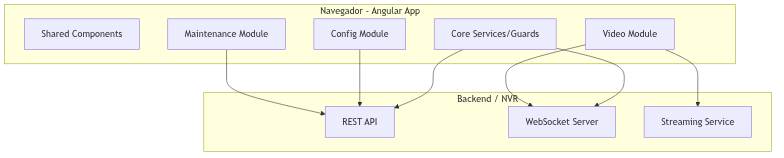
\includegraphics[width=0.85\textwidth]{figures/angular_components.png}
  \caption{Diagrama de components de l'arquitectura de l'aplicació Angular i la seva integració amb el backend.}
  \label{fig:angular_components}
  \small Font: Elaboració pròpia.
\end{figure}

\subsection{Arquitectura Modular i Standalone Components}
S'ha eliminat l'ús de mòduls clàssics d'Angular en favor dels \textit{Standalone Components}. Això redueix el \textit{boilerplate} del codi i millora el temps de càrrega de l'aplicació (\textit{lazy loading}), ja que només es descarreguen al navegador els components necessaris per a la vista actual (per exemple, el mòdul de configuració avançada no es carrega si l'usuari només vol veure vídeo).

L'organització d'aquests elements quant a dependències i estructura de mòduls es presenta gràficament a la Figura \ref{fig:angular_modules}.

\begin{figure}[!htbp]
  \centering
  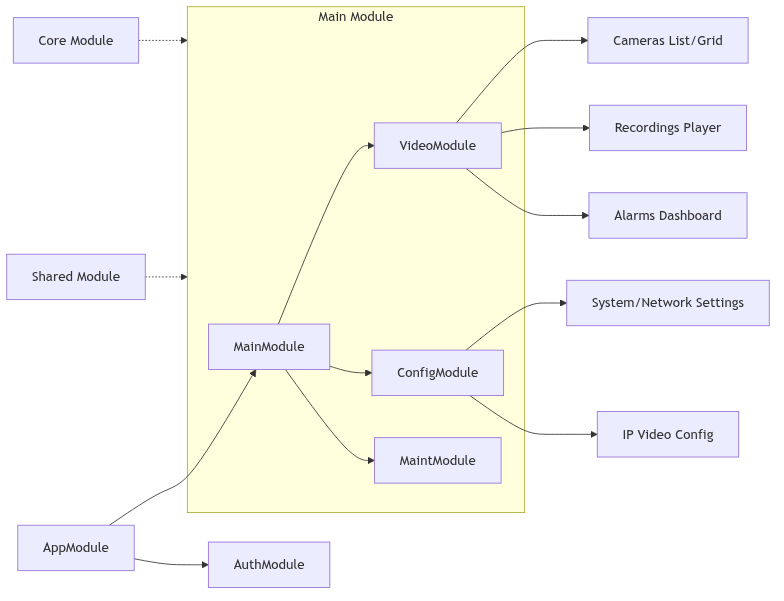
\includegraphics[width=0.75\textwidth, height=0.45\textheight, keepaspectratio]{figures/angular_modules.png}
  \caption{Diagrama de mòduls de l'aplicació Angular i relació amb els components compartits i serveis de la capa Core.}
  \label{fig:angular_modules}
  \small Font: Elaboració pròpia.
\end{figure}

\subsection{Gestió de l'Estat amb Angular Signals}
Aquest és un punt d'inflexió respecte a les versions anteriors del programari. Mentre que RxJS és excel·lent per a fluxos de dades complexos, \textbf{Angular Signals} permet una reactivitat granular \cite{learning_angular}.
\begin{itemize}
    \item \textbf{Eficiència:} En un sistema de vigilància on els estats de les càmeres canvien constantment, els \textit{Signals} asseguren que només es torni a renderitzar la part mínima de l'arbre del DOM afectada, reduint dràsticament l'ús de CPU al terminal del client.
    \item \textbf{Sincronització:} Els valors calculats (\textit{computed signals}) faciliten que la interfície s'adapti automàticament a canvis en el \textit{lock} de configuració o en l'estat de connectivitat informat pel \textit{Keep-alive}.
\end{itemize}

Dins d'aquest disseny de gestió d'estat reactiu, un dels reptes tècnics ha estat la modificació d'estructures de dades altament anidades zone-free sense trencar la detecció de canvis nativa. Angular Signals es basa en la comparació de valors per referència; per tant, mutar directament una propietat interna d'un objecte complex no dispararia la reactivitat del component. Per resoldre-ho, s'ha implementat un algorisme de manipulació profunda (\textit{deep copy} i \textit{deep access}) que clona l'objecte d'estat local completament, hi aplica la modificació en el camp editat dinàmicament (identificat pel camí de la propietat JSON de l'esquema), i finalment actualitza el Signal amb la nova referència (\texttt{configSignal.set(newConfig)}). Aquest disseny garanteix la immutabilitat de l'estat i evita defectes de renderitzat col·laterals.

A diferència de les arquitectures anteriors basades en \texttt{Zone.js}, que havien de revisar tot l'arbre de components davant qualsevol esdeveniment, l'ús de \textbf{Signals} permet que l'aplicació s'apropi a un model \textit{Zone-less} (amb l'ús puntual de \texttt{NgZone} per a operacions concretes que ho requereixen, com ara els temporitzadors del servei de \textit{keep-alive}). Això és especialment crític en la visualització de vídeo: el fet que arribin metadades cada 100ms sobre el bitrate no provoca que es torni a avaluar tota la interfície, sinó només l'etiqueta de text específica, alliberant cicles de CPU del terminal per dedicar-los exclusivament a la descodificació de vídeo H.265.

\section{El Motor Schema-Driven}
El component més innovador del sistema és el motor de configuració dinàmic. Aquest motor permet desacoblar totalment el desenvolupament del \textit{frontend} de l'evolució del \textit{firmware}.

\subsection{Lògica de funcionament}
En lloc de programar pantalles de configuració estàtiques, s'ha creat un intèrpret que segueix aquest flux:
\begin{enumerate}
    \item \textbf{Recepció del Schema:} El gravador envia un fitxer JSON que descriu les propietats (tipus de dades, límits, valors per defecte i dependències).
    \item \textbf{Parseig:} El servei \texttt{ConfigInputComponent} processa la metadada i mapeja cada propietat a un component visual (un \textit{toggle} per a booleans, un \textit{slider} per a sensibilitat, etc.).
    \item \textbf{Manipulació de camins:} S'utilitzen utilitats de \textit{Deep Access} per llegir i escriure en estructures d'objectes anidats (ex: \texttt{config.io.outputs[0].task}), garantint que l'enviament de tornada al servidor sigui un node vàlid.
\end{enumerate}

Aquest enfocament és especialment valuós quan s'introdueixen noves funcionalitats a \textbf{la-video-engine} o \textbf{la-core-alarm}. En lloc de programar una nova vista a Angular, el servei de backend simplement actualitza el seu esquema de dades i el \textit{frontend} el renderitza automàticament, reduint el temps de \textit{time-to-market} de noves versions del firmware.

És important destacar que el servei \textbf{la-core-legacy} és el responsable de generar aquest esquema dinàmic. El servei inspecciona les capacitats del maquinari (nombre de canals de vídeo, tipus de ports instal·lats) i construeix el diccionari de metadades JSON en temps real. Això permet que una mateixa versió de la interfície web sigui capaç de gestionar tant un gravador compacte de 4 càmeres com una unitat de rack de 64 càmeres, ja que el \textit{frontend} no té el nombre d'interfícies codificat de manera estàtica, sinó que es limita a renderitzar allò que \textbf{la-core-legacy} li indica.

Un dels reptes d'aquest disseny és la \textbf{tolerància a errors en l'esquema}. S'ha implementat una lògica de \textit{fail-safe} al frontend: si \textbf{la-core-legacy} envia un node de configuració amb un tipus no reconegut o amb paràmetres fora de rang, el motor no bloqueja el renderitzat de la resta de la pàgina. En lloc d'això, substitueix el component defectuós per un avís visual de 'Paràmetre no compatible', permetent que l'operador continuï treballant amb la resta del sistema sense patir un tancament inesperat de l'aplicació.

\section{Disseny de la Persistència i dades}
Tot i que el sistema és principalment una interfície de gestió, l'arquitectura preveu la persistència en dos nivells:
\begin{itemize}
    \item \textbf{SQLite3:} Utilitzada en el costat del servidor (\textit{backend embedded}) per a la gestió ràpida de l'historial d'alarmes i la configuració persistent dels usuaris.
    \item \textbf{Estratègia de Buffering:} El \textit{frontend} gestiona un estat local temporal per permetre a l'usuari realitzar múltiples canvis i validar-los abans d'adquirir el \textit{lock} i enviar la configuració final al maquinari.
\end{itemize}

\subsection{Model de dades de l'aplicació}
Per tal de representar la correspondència i relació entre les diferents estructures de dades que es reben de l'API (com ara Càmeres, Codecs, Presets o Alarmes), s'ha elaborat un model d'entitats representat en el diagrama de classes de la Figura \ref{fig:class_diagram}. Cal destacar que el model de la classe \texttt{Camera} està dissenyat per reflectir exactament l'estructura tipada del \textit{frontend} en TypeScript, incloent l'objecte imbricat \texttt{ipConfig}, el qual conté camps clau com \texttt{manufacturer} i \texttt{model}. Aquests camps són essencials per a la renderització correcta de les taules de manteniment i la generació d'informes tècnics d'estat de l'equip.

\begin{figure}[!htbp]
  \centering
  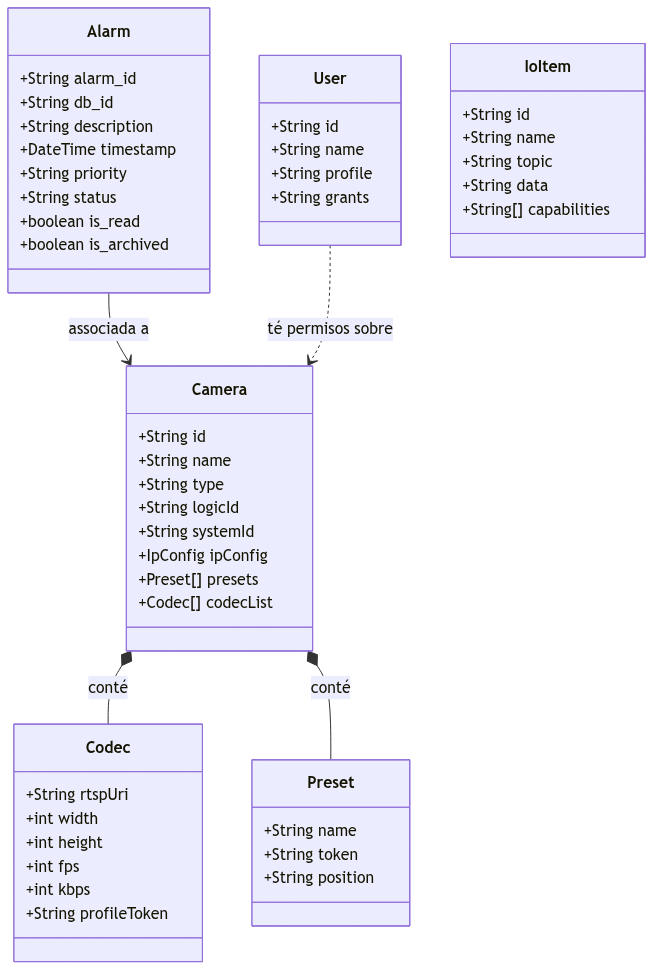
\includegraphics[width=0.75\textwidth, height=0.45\textheight, keepaspectratio]{figures/class_diagram.png}
  \caption{Diagrama de classes de les entitats principals del sistema WebCoreView.}
  \label{fig:class_diagram}
  \small Font: Elaboració pròpia.
\end{figure}